\chapter{The Discrete Fourier Transform} \label{ch:DFT}
In this chapter the discrete Fourier transform (DFT) is defined. Then a faster method of computing the DFT the fast Fourier transform (FFT) is derived and the discrete short-time Fourier transform is introduced as a method to analyse the frequency content of shorter segments of a signal.\\ 
As mentioned in \autoref{sec:ParametersAudioRecognition}, when analysing music, it can be beneficial to look at a signal in the frequency domain. A continuous signal can be transformed into the frequency domain by using the Fourier transform. 
\\
The Fourier transform only works on continuous signals, however it is possible to define the discrete Fourier transform, which can be applied for discrete signals. 

\begin{definition}{The Discrete Fourier Transform}
    The DFT, transforms a discrete signal $f$ in the time domain with $N$ terms, into a discrete sequence $F$ in the frequency domain also with $N$ terms, which is defined as: 
    \begin{align*}
        F[k]=\sum^{N-1}_{n=0}f[n]e^{-2jnk\pi/N}\quad \text{for } k=0, 1, ..., N-1,\, N \in \mathbb{N}_0.
    \end{align*}
    \cite[5]{rao2011fast}
    \label{def:DFT_definiton}
\end{definition}
The discrete signal $f$ and $F$ can be expressed as the following single vectors 
\begin{align*}
    \textbf{x}=
    \begin{bmatrix}
    f[0]\\f[1]\\ \vdots \\ f[N-1]
    \end{bmatrix},
    \quad \textbf{y}=
    \begin{bmatrix}
    F[0]\\F[1]\\ \vdots \\ F[N-1]
    \end{bmatrix}
\end{align*}
where $\textbf{x} \in \mathds{R}^{N}$ and $\textbf{y} \in \mathds{C}^{N}$. 
\\
In the following theorem it is shown, how the DFT can be represented as an matrix transformation.

\begin{theorem}{The Discrete Fourier Transform as a Matrix Transformation}
    By defining
    \begin{align*}
        W_N=e^{-2j\pi/N},
    \end{align*}
    which is called the twiddle factor. Then the DFT can be written as:
    \begin{align*}
        F[k]=\sum^{N-1}_{n=0}f[n]W_N^{nk}\quad \text{for } k=0, 1,...  N-1.
    \end{align*}
    From this the $N\times N$ $DFT_N$ matrix is defined as:
    \begin{align*}
        DFT_N=
        \begin{bmatrix}
             W_N^{0\cdot0} & W_N^{0\cdot1} & W_N^{0\cdot2} & \hdots & W_N^{0(N-1)} \\
             W_N^{1\cdot0} & W_N^{1\cdot1} & W_N^{1\cdot2} & \hdots & W_N^{1(N-1)} \\
             W_N^{2\cdot 0} & W_N^{2\cdot1} & W_N^{2\cdot2} & \hdots & W_N^{2(N-1)} \\
             \vdots & \vdots & \vdots & \ddots & \vdots \\
             W_N^{(N-1)0} & W_N^{(N-1)1} & W_N^{(N-1)2} & \hdots & W_N^{(N-1)(N-1)} \\
         \end{bmatrix}.
    \end{align*}
    The DFT of a vector $\textbf{x}$ can then be expressed as the matrix transformation
    \begin{align*}
        \textbf{y}=DFT_N\textbf{x}.
    \end{align*}
    \cite[10]{rao2011fast}
    \label{DFTasMatrixTransform}
\end{theorem}
Since the DFT can be expressed as a matrix transformation by Theorem \ref{the:linearityMatrixTransformation} the DFT is a linear transform.
\noindent In the following an example, using Theorem \ref{DFTasMatrixTransform} for $DFT_N$ for $N=1,\,2,\,4$.
\begin{example}{$DFT_N$}
    Due to some properties of symmetry and that $W_N^{kN}$ for $k\in \mathbb{R}$ is a value on the unit circle in the $z$-plane, $DFT_N$ can be determined.
    Since $W_N^{kN}$ is a value on the unit circle in the $z$-plane, it can be seen that $W_N^{N}=1$, $W_N^{N/4}=-j$, $W_N^{N/2}=-1$ and $W_N^{3N/4}=j$.\\
    Using the above to calculate $DFT_1$ and $DFT_2$ yields 
    \begin{align*}
     DFT_1 = \begin{bmatrix}
     W_1^{0\cdot0}
     \end{bmatrix}
     =
     \begin{bmatrix}
     1
     \end{bmatrix}\quad \text{and}\quad      DFT_2 =  
     \begin{bmatrix}
     1 & 1\\
     1 & -1
     \end{bmatrix}.
    \end{align*}
    From this it can be seen that $DFT_1$ and $DFT_2$ are real matrices, however these are the only real matrices\\
    By calculating $DFT_4$
    \begin{align*}
     DFT_4 = 
     \begin{bmatrix}
     1 & 1 & 1 & 1\\
     1 & -j & -1 & j\\
     1 & -1 & -1 & 1\\
     1 & j & 1 & -j
     \end{bmatrix},
    \end{align*}
    it can be seen that it is a complex matrix.
\end{example}
To compute the DFT, it is necessary to do $N^2$ computations. To reduce the amount of computations, the fast Fourier transform is used.
\section{The Fast Fourier Transform}
The Fast Fourier Transform (FFT) is a method of reducing the number of computations needed to calculate the DFT. This can be accomplished by reducing the DFT matrix to a product of sparse matrices. 
To do so the following theorem is needed.

\begin{theorem}{The DFT when $N$ is even}
    Let $\mathbf{y}=DFT_{N}\mathbf{x}$ be the $N$-point DFT of $\mathbf{x}$ where $N$ is even and let $D_{N/2}$ be an $(N/2)\times(N/2)$ diagonal matrix with entries 
    \begin{align}
        (D_{N/2})_{n,n}=W_N^n \quad \text{for} \quad 0 \leq n< N/2.
        \label{eq:DFTDiagonal}
    \end{align}
    It can then be written as:
    \begin{align*}
         \mathbf{y_1}&=DFT_{N/2}\mathbf{x}^{(e)}+D_{N/2}DFT_{N/2}\mathbf{x}^{(o)}\\ 
         \mathbf{y_2}&=DFT_{N/2}\mathbf{x}^{(e)}-D_{N/2}DFT_{N/2}\mathbf{x}^{(o)}.
    \end{align*}
    Where $\mathbf{y_1}$ is the first half $N/2$ entries of $\mathbf{y}$ and $\mathbf{y_2}$ is the second half of entries and $\mathbf{x}^{(e)}$ and $\mathbf{x}^{(o)}$ are the even and odd entries of $\mathbf{x}$ respectively. Hence $\mathbf{x}^{(e)},\mathbf{x}^{(o)}\in \mathds{R}^{N/2}$ and $\mathbf{y_1},\mathbf{y_2}\in \mathds{C}^{N/2}$. \cite[67]{ryan2019linear}
    \label{theo:DFT_N_even}
\end{theorem}
\begin{proof}{The DFT when $N$ is even}
From \autoref{def:DFT_definiton}:
    \begin{align*}
         F[k]&=\sum^{N-1}_{n=0}f[n]W_N^{nk}.\\
        \intertext{The sum of the DFT can be split into two sums, an even and an odd part.}
        &=\sum^{N/2-1}_{r=0}f[2r]W_N^{2rk}+\sum^{N/2-1}_{r=0}f[2r+1]W_N^{(2r+1)k}\\
        \intertext{This can be rewritten to $W_N^2$ and moving the constant $W_N^k$ out of the sum}
        &=\sum^{N/2-1}_{r=0}f[2r](W_N^2)^{rk}+W_N^k\sum^{N/2-1}_{r=0}f[2r+1](W_N^2)^{rk}.\\
        \intertext{Note that $W_N$ is defined as $e^{-2j\pi/N}$, hence}
        W_N^2 &= \exp\left(\frac{-j2(2\pi)}{N}\right) = \exp\left(\frac{-j2\pi}{N/2}\right) = W_{N/2}.\\
        \intertext{Thereby it yields:}
        F[k] &= \sum^{N/2-1}_{r=0}f[2r]W^{rk}_{N/2}+W^k_N\sum^{N/2-1}_{r=0}f[2r+1]W^{rk}_{N/2}.
    \end{align*}
    Using \eqref{eq:DFTDiagonal} where $0 \leq k < N/2$ the first half can be written as:
     \begin{align*}
        \mathbf{y_1}=DFT_{N/2}\mathbf{x}^{(e)}+D_{N/2}DFT_{N/2}\mathbf{x}^{(o)}.
     \end{align*}
    If $k$ is limited to $0 \leq k < N/2$, then the second half $\mathbf{y_2}$ of the DFT can be processed using the same method as in the first half $\mathbf{y}_1$:
    \begin{align*}
        F[k+N/2] &= \sum^{N-1}_{n=0}f[n]W_N^{n(k+N/2)}\\
        &=\sum^{N/2-1}_{r=0}f[2r]W_N^{2r(k+N/2)}+\sum^{N/2-1}_{r=0}f[2r+1]W_N^{(2r+1)(k+N/2)}\\
        &=\sum^{N/2-1}_{r=0}f[2r](W_N^2)^{r(k+N/2)}+W_N^{k+N/2}\sum^{N/2-1}_{r=0}f[2r+1](W_N^2)^{r(k+N/2)}\\
        W_N^{N/2}&=\exp\left(\frac{-j2\pi}{N}\frac{N}{2}\right)=\exp\left(-j\pi\right)=-1\\
        F[k+N/2] &=\sum^{N/2-1}_{r=0}f[2r]W_{N/2}^{r(k+N/2)}-W_N^{k}\sum^{N/2-1}_{r=0}f[2r+1]W_{N/2}^{r(k+N/2)}.
    \end{align*}
    This can be written using \eqref{eq:DFTDiagonal} where $0 \leq k < N/2$ as:
    \begin{align*}
        \mathbf{y_2}=DFT_{N/2}\mathbf{x}^{(e)}-D_{N/2}DFT_{N/2}\mathbf{x}^{(o)}.
     \end{align*}
     \cite[67]{ryan2019linear}
\end{proof}
From Theorem \ref{theo:DFT_N_even} the DFT of $\textbf{x}$ can be expressed as: 
\begin{align*}
    \mathbf{y}=
    \begin{bmatrix}
        \mathbf{y_1}\\
        \mathbf{y_2}
    \end{bmatrix}
    &=
    \begin{bmatrix}
        DFT_{N/2} & D_{N/2}DFT_{N/2} \\
        DFT_{N/2} & -D_{N/2}DFT_{N/2}
    \end{bmatrix}
    \begin{bmatrix}
        \mathbf{x}^{(e)} \\
        \mathbf{x}^{(o)}
    \end{bmatrix}\\
    &=
    \begin{bmatrix}
        I_{N/2} & D_{N/2} \\
        I_{N/2} & -D_{N/2}
    \end{bmatrix}
    \begin{bmatrix}
        DFT_{N/2} & \mathbf{0} \\
        \mathbf{0} & DFT_{N/2}
    \end{bmatrix}
    \begin{bmatrix}
        \mathbf{x}^{(e)} \\
        \mathbf{x}^{(o)}
    \end{bmatrix}.
\end{align*}
If $N/2$ is even then $DFT_{N/2}$ can be factored into:
\begin{align*}
        \mathbf{y}=
    \begin{bmatrix}
        I_{N/2} & D_{N/2} \\
        I_{N/2} & -D_{N/2}
    \end{bmatrix}
    \begin{bmatrix}
        I_{N/4} & D_{N/4} & \mathbf{0} & \mathbf{0} \\
        I_{N/4} & -D_{N/4} & \mathbf{0} & \mathbf{0} \\
        \mathbf{0} & \mathbf{0} & I_{N/4} & D_{N/4}  \\
        \mathbf{0} & \mathbf{0} & I_{N/4} & -D_{N/4} \\
    \end{bmatrix}\times\\
    \begin{bmatrix}
        DFT_{N/4} & \mathbf{0} & \mathbf{0} & \mathbf{0} \\
        \mathbf{0} & DFT_{N/4} & \mathbf{0} & \mathbf{0} \\
        \mathbf{0} & \mathbf{0} & DFT_{N/4} & \mathbf{0} \\
        \mathbf{0} & \mathbf{0} & \mathbf{0} & DFT_{N/4} \\
    \end{bmatrix}
    \begin{bmatrix}
        \mathbf{x}^{(ee)} \\
        \mathbf{x}^{(eo)} \\
        \mathbf{x}^{(oe)} \\
        \mathbf{x}^{(oo)}
    \end{bmatrix},
\end{align*}
where $\mathbf{x}^{(e)}$ and $\mathbf{x}^{(o)}$ are split into even and odd parts.  
If $N$ is limited to be $N=2^L$, where $L$ is an positive integer. Then $DFT_N$ can be factored $L=\log_2 N$ times. When factorising $\log_2 N$ times, the final matrix becomes a diagonal matrix with entries $DFT_1=[1]$, which is the identity matrix. Hence it is only necessary to factor the matrix $\log_2(N) - 1$ times. \cite[68-69]{ryan2019linear}\\
This can be generalised as
\begin{align*}
    DFT_N=\prod_{k=1}^{\log_2 N}\left(
    \begin{bmatrix}
    I_{N/2^k}  & D_{N/2^k}  & \mathbf{0} & \mathbf{0} & \hdots & \mathbf{0} & \mathbf{0}\\
    I_{N/2^k}  & -D_{N/2^k} & \mathbf{0} & \mathbf{0} & \hdots & \mathbf{0} & \mathbf{0}\\
    \mathbf{0} & \mathbf{0} & I_{N/2^k}  & D_{N/2^k}  & \hdots & \mathbf{0} & \mathbf{0}\\
    \mathbf{0} & \mathbf{0} & I_{N/2^k}  & -D_{N/2^k} & \hdots & \mathbf{0} & \mathbf{0}\\
    \vdots     & \vdots     & \vdots     & \vdots     & \ddots & \vdots     & \vdots    \\
    \mathbf{0} & \mathbf{0} & \mathbf{0} & \mathbf{0} & \hdots & I_{N/2^k}  & D_{N/2^k} \\
    \mathbf{0} & \mathbf{0} & \mathbf{0} & \mathbf{0} & \hdots & I_{N/2^k}  & -D_{N/2^k}
    \end{bmatrix}
    \right)P.
\end{align*}
To split the input vector into the even and odd parts of the transformation, a $N\times N$ permutation matrix $P$, is used. To illustrate how to determine $P$, the following example is used. 

\begin{example}{Bit Reversal}
    A $DFT_8$ can be factored $\log_2 8-1=2$ times. Which means that the input vector needs to be split into odd and even values twice. This is illustrated below:
    \begin{align*}
        \begin{bmatrix}
            x_0 \\
            x_1 \\
            x_2 \\
            x_3 \\
            x_4 \\
            x_5 \\
            x_6 \\
            x_7
        \end{bmatrix}
        \rightarrow
        \begin{bmatrix}
            x_0 \\
            x_2 \\
            x_4 \\
            x_6 \\
            x_1 \\
            x_3 \\
            x_5 \\
            x_7
        \end{bmatrix}
        \rightarrow
        \begin{bmatrix}
            x_0 \\
            x_4 \\
            x_2 \\
            x_6 \\
            x_1 \\
            x_5 \\
            x_3 \\
            x_7
        \end{bmatrix}.
    \end{align*}
    It is observed that, if using the binary representation of the indexes of the first vector, then bit reversing it, the indexes of the last vector is obtained. For instance the binary representation of $3=011_2$ and when reversing the bits, $110_2=6$. Therefore, the sixth index will be placed in third index of the final vector.
    
    To represent the example as a matrix, the values from the first vector need to be transformed into the third vector by multiplying with the following matrix:
    \begin{align*}
        P&=
        \begin{bmatrix}
            1 & 0 & 0 & 0 & 0 & 0 & 0 & 0\\
            0 & 0 & 0 & 0 & 1 & 0 & 0 & 0\\
            0 & 0 & 1 & 0 & 0 & 0 & 0 & 0\\
            0 & 0 & 0 & 0 & 0 & 0 & 1 & 0\\
            0 & 1 & 0 & 0 & 0 & 0 & 0 & 0\\
            0 & 0 & 0 & 0 & 0 & 1 & 0 & 0\\
            0 & 0 & 0 & 1 & 0 & 0 & 0 & 0\\
            0 & 0 & 0 & 0 & 0 & 0 & 0 & 1\\
        \end{bmatrix}\\
        &=\begin{bmatrix}
        \mathbf{e}_1 & \mathbf{e}_5 & \mathbf{e}_3 & \mathbf{e}_7 & \mathbf{e}_2 & \mathbf{e}_6 & \mathbf{e}_4 & \mathbf{e}_8
        \end{bmatrix}.
 \end{align*}
   As seen $P$ is represented as a $N \times N$ matrix, where the columns contains unit vectors $\mathbf{e}_{i+1}$ respectively, where $i$ is the bit reversed index number from $0$ to $N-1$.
    \label{exa:bitreverse}
\end{example}
From Example \ref{exa:bitreverse}, it can be generalised that $P$ is represented as a $N \times N$ matrix, where the columns contain the unit vector $\mathbf{e}_{i+1}$ from the bit reversed vector respectively. \\

When making the Fourier transform of a signal the signal is transformed from the time domain to the frequency domain. Making this transformation the frequencies are known from the entire signal, but its not known when these frequencies occur. To analyse at which time frequencies occur, the discrete short-time Fourier transform can be relevant to use. 

\section{The Discrete Short-Time Fourier Transform}

\indent Dealing with audio signals it can be desirable to use discrete short-time Fourier transform (DSTFT), because it can be used to quantify the change of a nonstationary signal's frequency and phase content over time. 
DSTFT can be seen as selecting a segment of a signal using a windowing function, and then Fourier transform it. Using a windowing function to a signal is a convolution of an input signal and an impulse response. This is defined as
\begin{definition}{Discrete Convolution}
    \begin{align*}
        y[n]=f[n]*w[n]=\sum_{m=-\infty}^{\infty}f[m]w[n-m],
    \end{align*}
    where $y[n]$ is the output response of the convolution \cite{spectralaudioCH2}.
\end{definition}
The formal definition for the discrete short-time Fourier transform (DSTFT) is 
\begin{align*}
    F_w[n,k]=\sum^{\infty}_{m=-\infty}f[m]w[n-m]e^{-j\frac{2\pi k}{N}  m},\quad \text{for } k=0, 1,...  N-1,
\end{align*}
where $f[n]$ is the input signal at time $n$, $w[n]$ is a window function with length $M$, $F_w[n,k]$ is the Fourier transform of the output response for the convolution $(f*w)[n]$, within the length $M$ of the time window. The length of each frame $M$ should be less than or equal to the length of the signal $N$ $w[n]$\cite[56]{layer2015signal}. 
\\
Time windows have different properties, in general it is a way to consider a smaller segment of the whole input signal. Each segment has the length $M$ and can be considered as a frame of the input signal, where $n$ is the number of a given frame.

\begin{figure}[H]
    \centering
    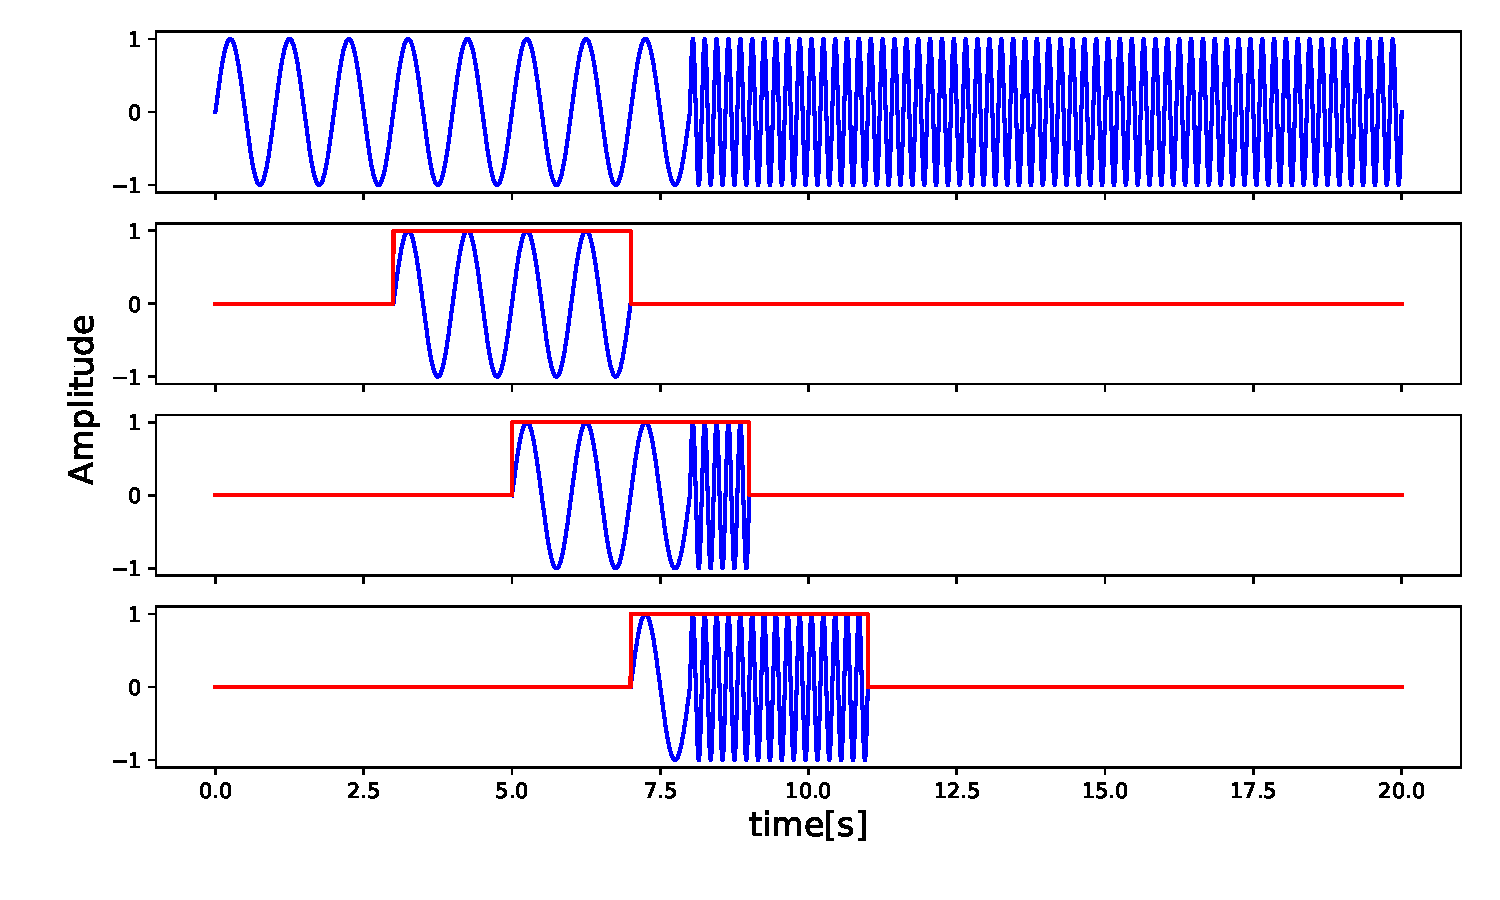
\includegraphics[width=\textwidth]{figures/overlapfigure.pdf}
    \caption{Illustrates "framing" of the original signal shown in the top, where frame $n$, $n+1$ and $n+2$ is shown. The original signal consist of two subsequent sinusiods of frequency 1 Hz and 5 Hz, and the applied time window is the rectangular window, with a window length of $M=4$ and 50\% overlap from a frame to another. }
    \label{fig:overlap}
\end{figure}


Applying time windows, a given frame $n$ of the signal is nonzero in a specified time interval, and null otherwise, as shown in \autoref{fig:overlap}. There exist different types of window functions, which makes it possible to choose the most beneficial, in different cases. Often a window function is symmetrical and has the highest value around the middle of the interval. \\
%In figure ?? a signal and the Fourier transform of the windowed version shown. In the figure a bell shaped time window is applied, and there is shown different segments of the signal. 
One type of window function is the rectangular window which is defined as:
\begin{definition}{Rectangular window}
\begin{align*}
    w_R(n)=
    \begin{cases}
    1, & -\frac{M-1}{2}\leq n \leq \frac{M-1}{2} \\
    0, & \text{otherwise}
    \end{cases}
\end{align*}
where $M$ is the length of the window in samples.
\end{definition}
The Fourier transform of $w_R(n)$ and $w_R(n)$ in time domain, are plotted in \autoref{fig: Rectangular}, where $M=21$, and centered at time $t=10$. 
\begin{figure}[H]
    \centering
    \begin{subfigure}[b]{.49\textwidth}
        \centering
        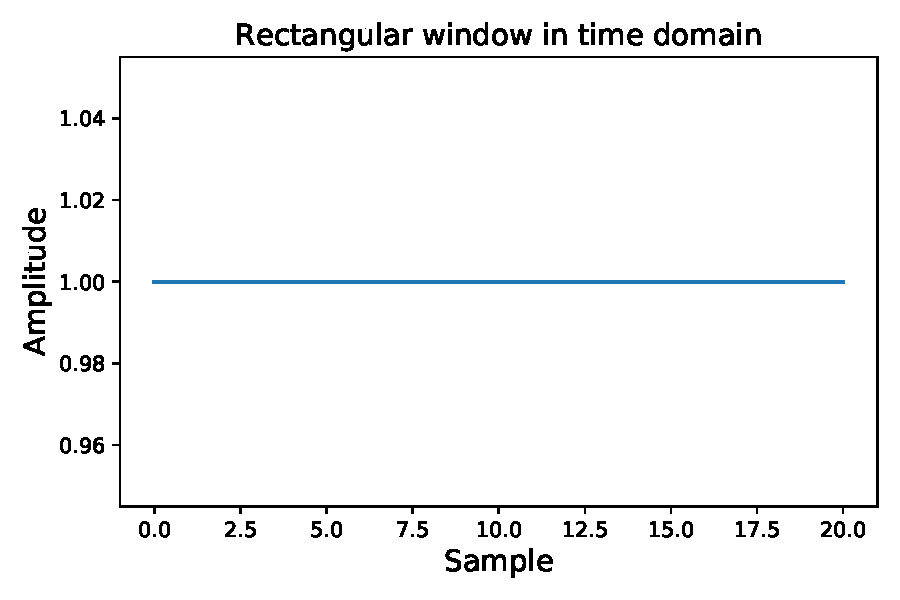
\includegraphics[width=\textwidth]{figures/RectangularTime.pdf}
         \caption{}
        \label{fig:RectangularTime}
    \end{subfigure}
    \begin{subfigure}[b]{.49\textwidth}
        \centering
        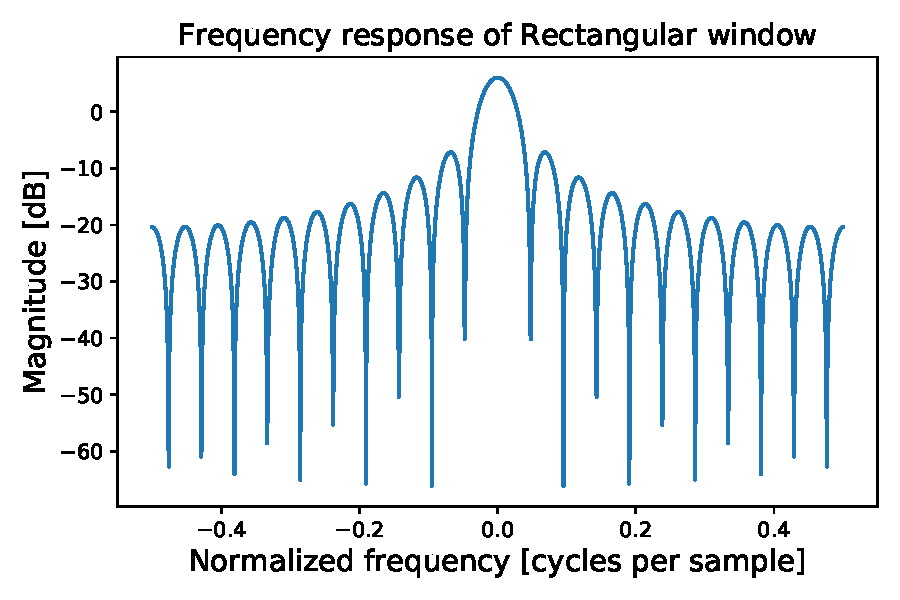
\includegraphics[width=\textwidth]{figures/RectangularFourier.pdf}
        \caption{}
        \label{fig:RectangularFourier}
    \end{subfigure}
\caption{Rectangular time window, centered at t=10 and window length $M=21$ and its Fourier transform.}
\label{fig: Rectangular}
\end{figure}

A commonly used type of time windows, is the time windows in the Hamming family. A Hamming window consists of a rectangular window multiplied by one period of cosine. 

\begin{definition}{Generalised Hamming window}
A generalised Hamming window is defined as followed.
\begin{align*}
    w_H(n)=w_R(n) \left(\alpha +2\beta \cos\left(\frac{2\pi n}{M}\right)\right),
\end{align*}
where $\alpha$ and $\beta$ are constants. 
\end{definition}

The different windows in the Hamming family have different parameters for $\alpha$ and $\beta$. 
One of these windows is called the Hanning window.
The Hanning window is defined by having the parameters $\alpha = \frac{1}{2} $ and $\beta = \frac{1}{4}$, hence
\begin{align*}
    w_H(n)&=w_R(n) \left(\frac{1}{2} + \frac{1}{2} \cos\left(\frac{2\pi n}{M}\right)\right) = w_R(n) \frac{1}{2}\left(1+\cos\left(\frac{2\pi n}{M}\right)\right)
\end{align*}
Using one of the fundamental trigonometric identities
\begin{align*}
    \cos^2(x)=\frac{1+\cos(2x)}{2},
\end{align*}
the expression for $w_H(n)$ above can be written as
\begin{align*}
    w_H(n)&=w_R(n)\cos^2\left(\frac{\pi n}{M}\right).
\end{align*}
Hence $w_H(n)$ can be defined as:
\begin{definition}{The Hanning time window}
   \begin{align*}
        w_H(n)=
    \begin{cases}
    \cos^2\left(\frac{\pi n}{M}\right), & -\frac{M-1}{2}\leq n \leq \frac{M-1}{2} \\
    0, & \text{otherwise}
    \end{cases}   
   \end{align*}
\end{definition}
The Fourier transform of $w_H(n)$ and $w_H(n)$ in time domain, are plotted in \autoref{fig: Hanning}, where $M=21$, and centered at time $t=10$.
\begin{figure}[H]
    \centering
    \begin{subfigure}[b]{.49\textwidth}
        \centering
        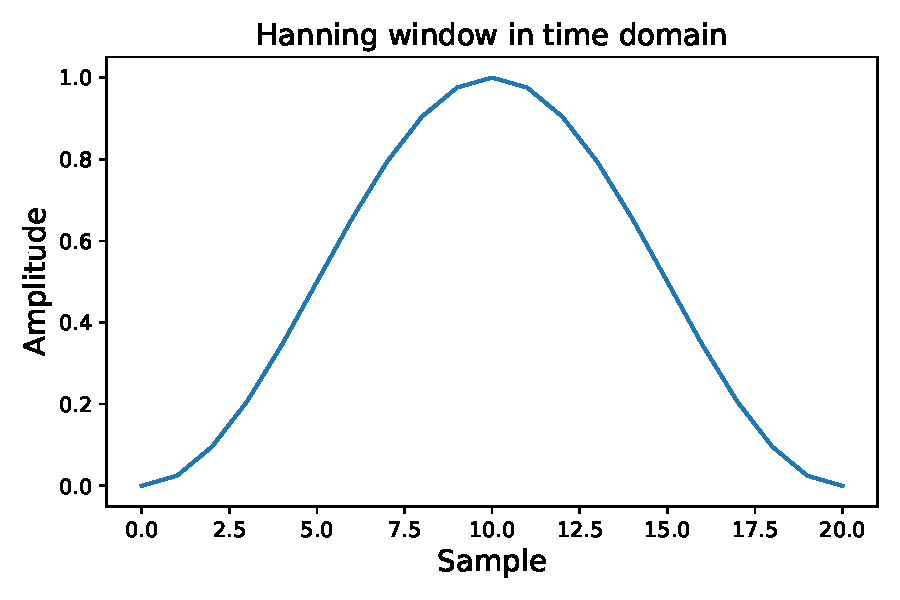
\includegraphics[width=\textwidth]{figures/HanningTime.pdf}
        \caption{}
        \label{fig:hanningtime}
    \end{subfigure}
    \begin{subfigure}[b]{.49\textwidth}
        \centering
        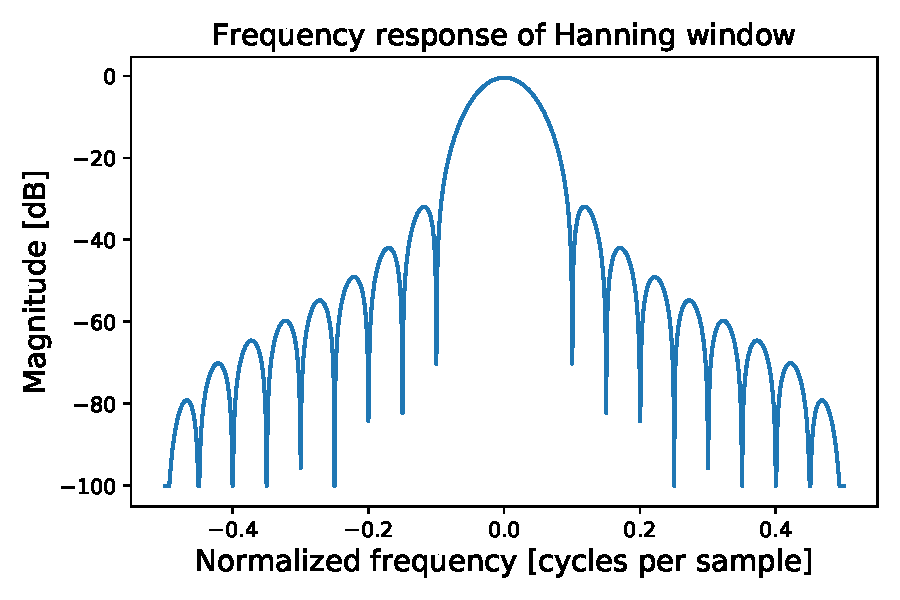
\includegraphics[width=\textwidth]{figures/HanningFourier.pdf}
        \caption{}
        \label{fig:hanningfourier}
    \end{subfigure}
\caption{Hanning time window and its Fourier transform}
\label{fig: Hanning}
\end{figure}
One of the differences, when comparing a Hanning window and the rectangular window, is that the Hanning window has faster roll-off of the side lobes, meaning that the side lobes are more attenuated. This can be seen by comparison of \autoref{fig:RectangularFourier} and \autoref{fig:hanningfourier}. When choosing a window function with faster roll-off, it minimises the risk of "crosstalk". Crosstalk is when a signal leakage from one channel or circuit to another, which can cause an unwanted effect. \\

In relation to the length $M$ of the time window, a narrow time window, will result in a good time resolution, but a worse frequency resolution. Therefore a wide time window will result in a better frequency resolution, but a worse time resolution. Hence it is not possible to attain high time resolution and high frequency resolution at the same time. 

The relation between the length of a time window, and the wide of its main lobe is described for a rectanglular and a Hanning window:

\begin{align*}
    \text{Rectangular window} = \frac{4\pi}{M} \\
    \text{Hanning window} = \frac{8\pi}{M}
\end{align*}
\cite{spectralaudioCH3}
\\
An ideal window requires a main lobe as narrow as possible and a fast roll-off\cite[56]{layer2015signal}. In relation to Hanning and rectangular windows, Hanning has low side lobes, but a twice as wide main lobe, meaning that applying a Hanning window results in a worse frequency resolution.
\\
With the knowledge of the relationship between length of time window, wide of lobes and resolution, a beneficial time window can be chosen to a given purpose.
In this project, the purpose is to be able to recognise a song, hence the input to the system can be some unknown content, in form of a recording. Here it can be beneficial to use a Hanning window, because it has a wide main lobe and low side lobes, hence a moderate resolution.


% \begin{definition}{The Constant Overlap-Add Property}
% A window function $w(n)$ has the COLA property if:
% \begin{align*}
%     \sum_{m=-\infty}^{\infty}w(n-m)=1,\quad \forall n \in \mathbb{Z}
% \end{align*} 
% \end{definition}

To visualise the STFT, spectrograms are often used. A spectrogram is a two dimensional representation of time, frequency and magnitude, which is represented by the squared magnitude $|F_w[n,k]|^2$.
\autoref{fig: spectrogram_of_C4}, shows a spectrogram of the tone C4, where the horizontal axis represents time, the vertical axis represents the frequency, and the intensity of color represents the value of the squared magnitude. On the figure it can be seen that the spectrum in general consist of the partial tones for C4. 

\begin{figure}[H]
    \centering
    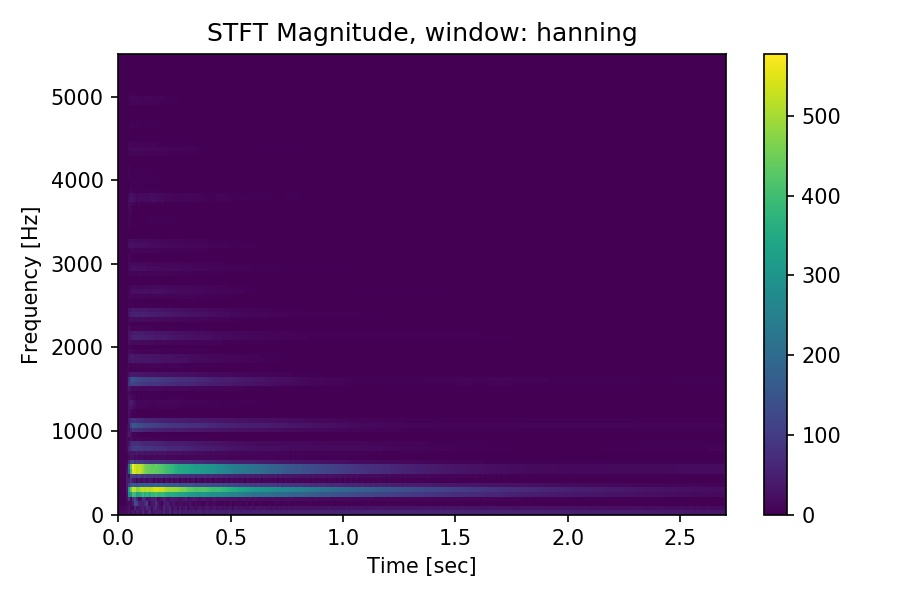
\includegraphics[width=0.7\textwidth]{figures/spectrogramC4hanning.jpg}
    \caption{A spectrogram of a $C_4$ tone, with a Hanning window }
    \label{fig: spectrogram_of_C4}
\end{figure}

A spectral analysis of an input signal results in a $F \times T$ matrix, where each column in the matrix is the frequency content of a given frame. This leads to the next chapter, where it will be described how to analyse, and find patterns in a matrix. 